\documentclass{zhvt-classic}

\zhvtset{
    grid_lines = false,
}

\title{印譜}
\ExplSyntaxOn
\mark_insert:nn { zhvt_chapter } { 卷一 }
\ExplSyntaxOff
\setcounter{page}{3}
\begin{document}
%\maketitle{}{}
~\vspace{-0.25\baselineskip}

\hfil 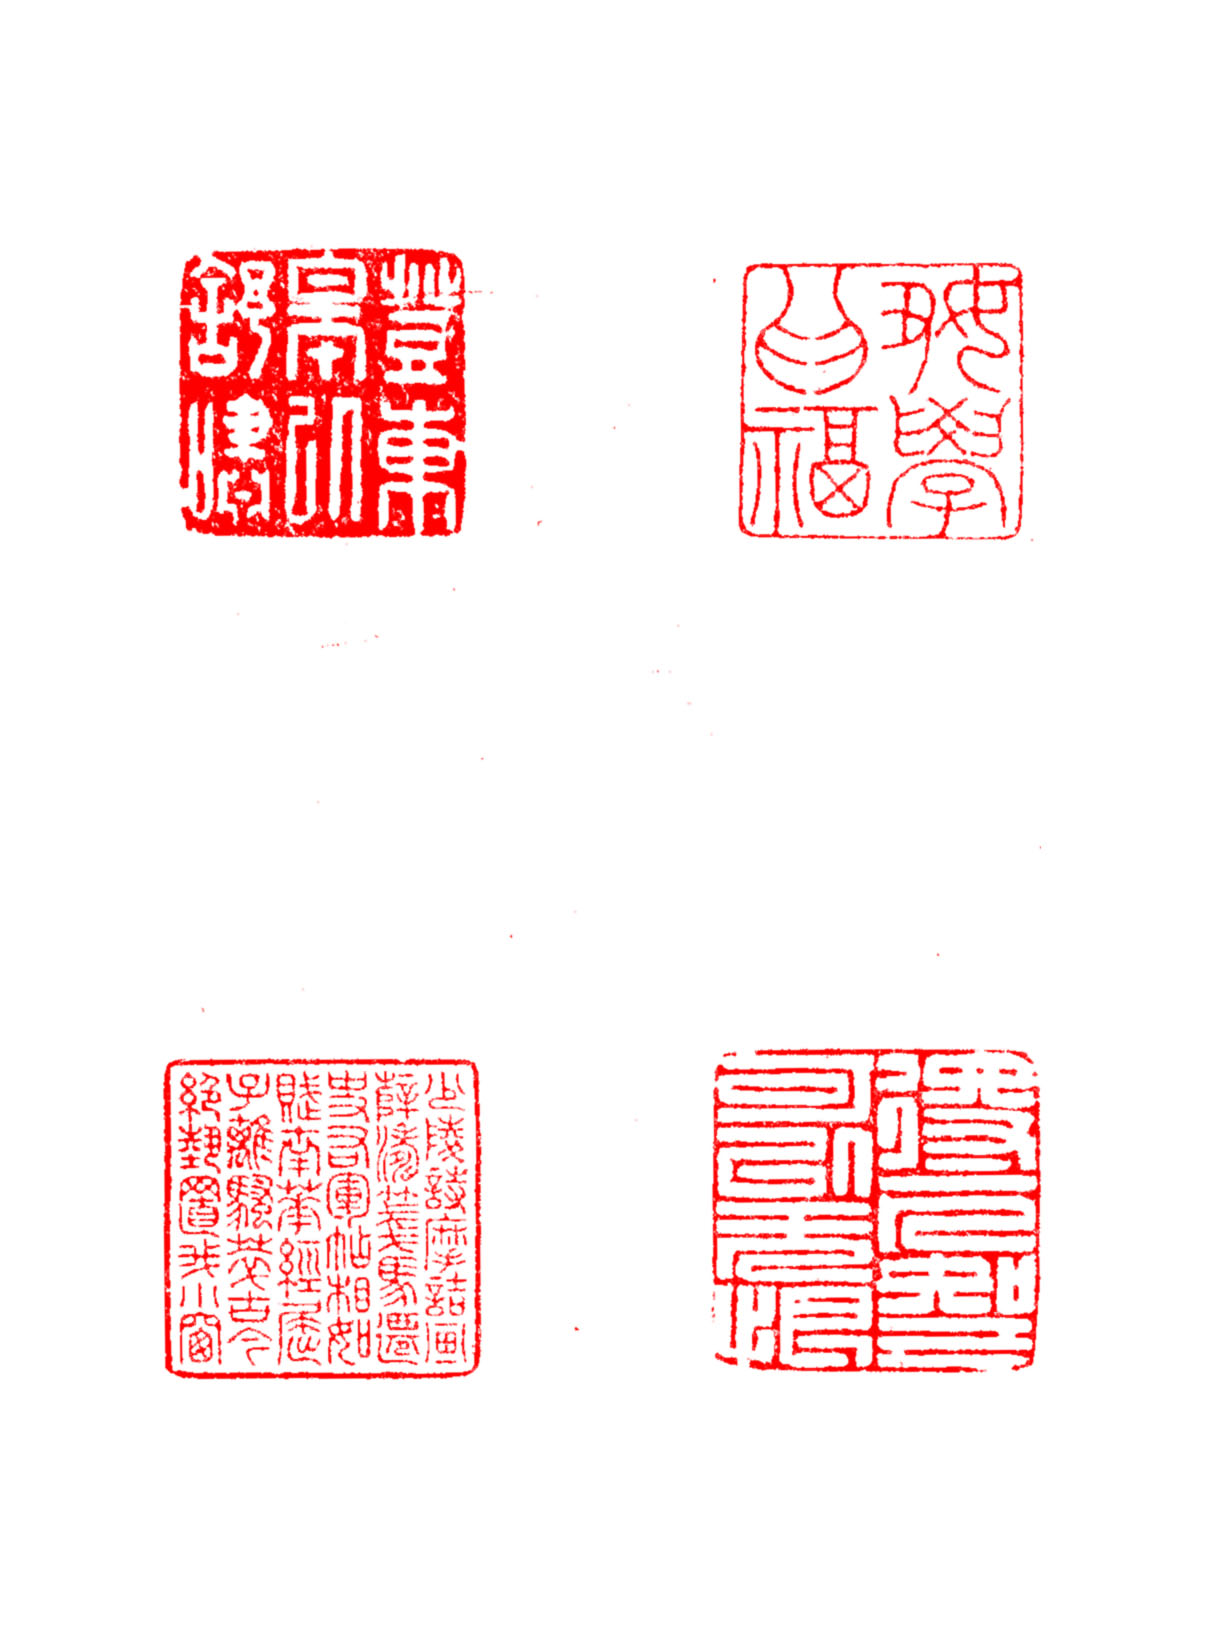
\includegraphics[angle=90]{stamp01}
\clearpage

好學爲福

得一人知己可以無恨

登東皋以舒嘯

少陵詩摩詰畫薛濤箋馬遷史友軍帖相如賦南華經屈子離騷萃古今絕藝置我小窗

\clearpage
~\vspace{-0.25\baselineskip}

\hfil 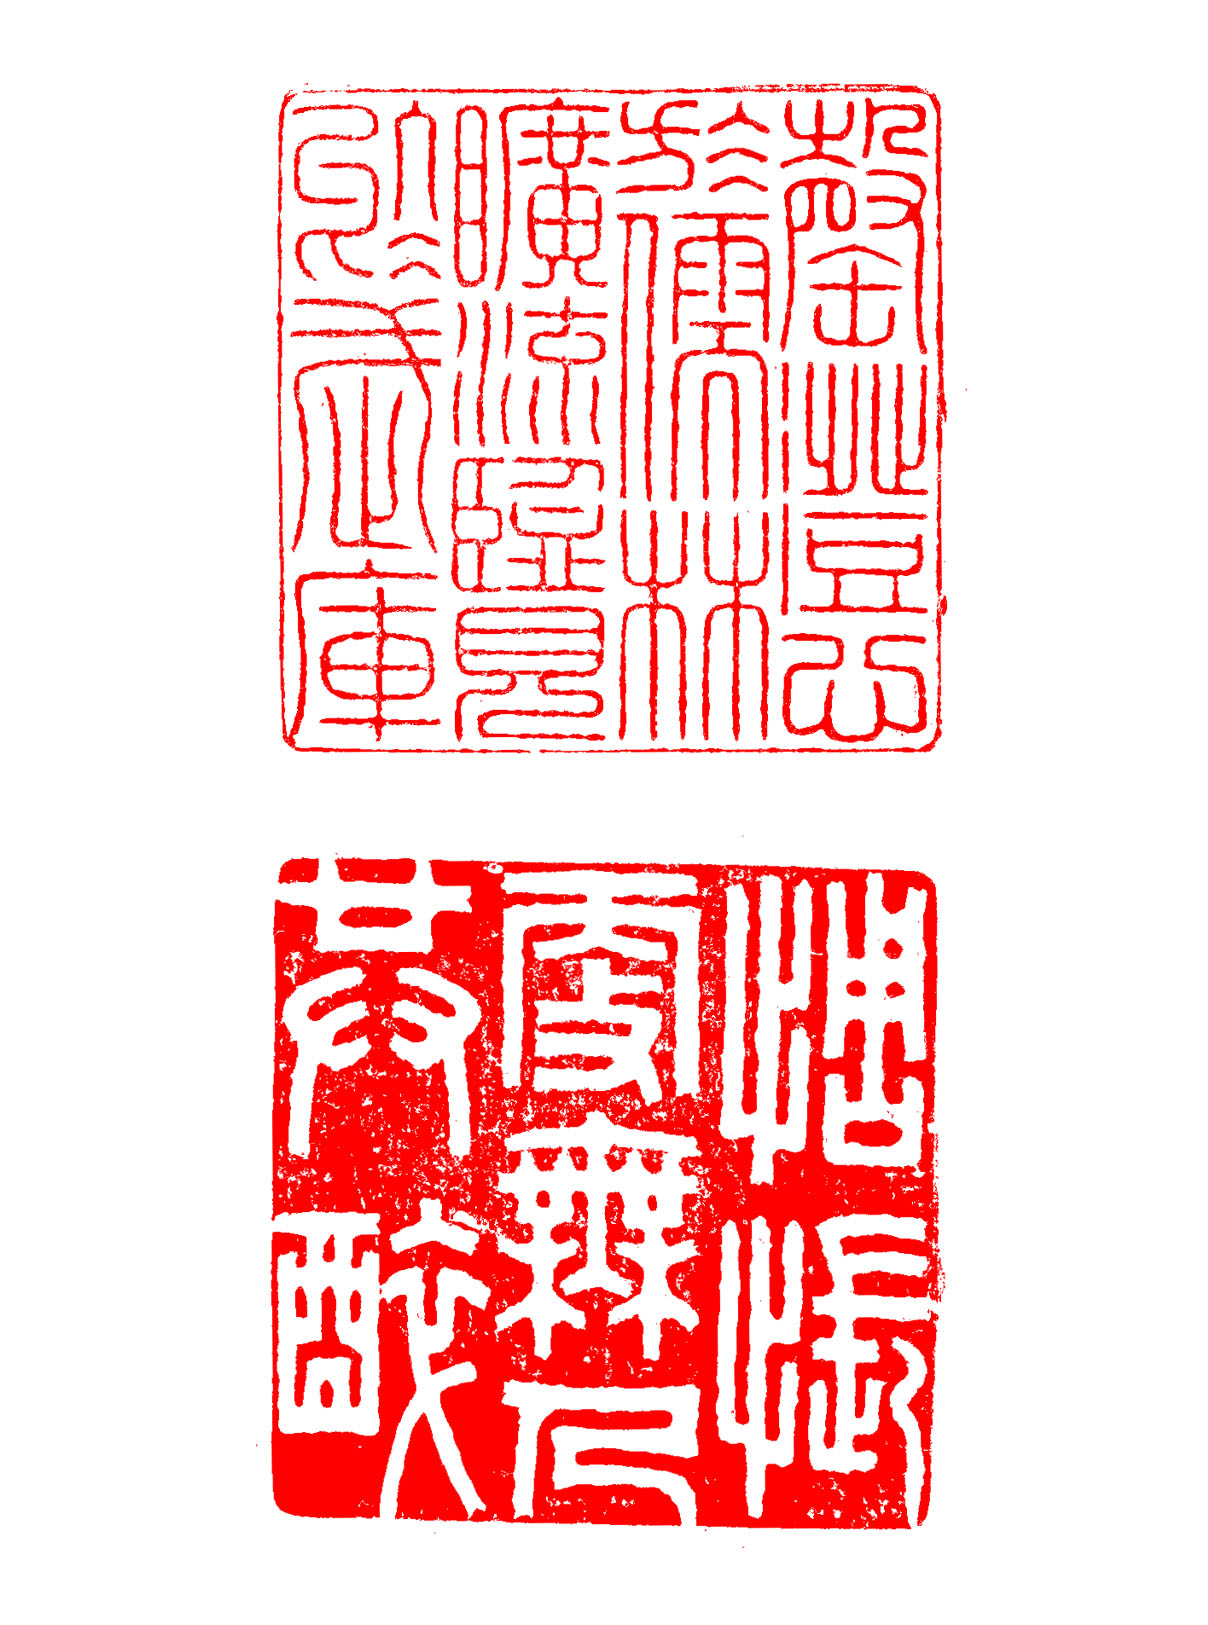
\includegraphics[angle=90]{stamp02}
\clearpage

罄澄心於儒林曠流覽於武庫

惆悵更無人共醉

\end{document}